\documentclass{beamer}
 
\usepackage[utf8]{inputenc}
\usepackage[brazil]{babel} % pacote portugues brasileiro
\usepackage{textpos}
\usepackage{hyperref}
\definecolor{blue(pigment)}{rgb}{0.2, 0.2, 0.6}
\hypersetup{
    colorlinks=true,
    linkcolor=blue(pigment),
    filecolor=magenta,      
    urlcolor=cyan,
}
\usetheme{Montpellier}
\usecolortheme{rose}
% \graphicspath{{../../../2021-1/DesWebBasico/aulas/fig/}}
% Layout da pagina
\hypersetup{pdfpagelayout=SinglePage}
 
%Information to be included in the title page:
\title[CSS]{Introdução ao CSS}
 \subtitle{Disciplina: Desenvolvimento de Sistemas com PHP}
\author{Juliana C. Silva}
\institute{Universidade Positivo}

\definecolor{UniGray}{RGB}{192,192,192}
\definecolor{nGray}{RGB}{220,220,220}

\setbeamercolor{block title}{use=structure,bg=UniGray}
\setbeamercolor{block body}{use=structure,bg=nGray}
\setbeamersize{text margin left=25pt,text margin right=25pt}
\setbeamertemplate{navigation symbols}{}%remove navigation symbols
 
% Configurando layout para mostrar codigos C++
\usepackage{listings}
\lstset{
  language=HTML,
  basicstyle=\ttfamily\small, 
  keywordstyle=\color{blue}, 
  stringstyle=\color{red}, 
  commentstyle=\color{red}, 
  extendedchars=true, 
  showspaces=false, 
  showstringspaces=false, 
  numbers=left,
  numberstyle=\tiny,
  breaklines=true, 
  backgroundcolor=\color{green!10},
  breakautoindent=true, 
  captionpos=b,
  xleftmargin=0pt,
}

\begin{document}
%------------------------------------------------------------------------------------------
\frame{\titlepage}
 
\addtobeamertemplate{frametitle}{}{%
\begin{textblock*}{100mm}(.8\textwidth,-1.45cm)
%\includegraphics[height=0.8cm,width=2.5cm]{logo_unicesumar.png}
\end{textblock*}
}

%--------------------------aula 4 des. app---------------------------------------------
\section{Introdução}
\begin{frame}{Recapitulando...}
Nas últimas aulas vimos:
  \begin{enumerate}
   \item Tags HTML;
   \item Elementos básicos HTML;
  \end{enumerate}
\end{frame}
%------------------------------------------------------------------------------------------
\begin{frame}
\frametitle{Roteiro} % Table of contents slide, comment this block out to remove it
\tableofcontents % Throughout your presentation, if you choose to use \section{} and \subsection{} commands, 
%these will automatically be printed on this slide as an overview of your presentation
\end{frame}
%-------------------------------------------------------------------------------
\begin{frame}{Introdução}
\begin{block}{CSS}
CSS é a sigla para o termo em inglês Cascading Style Sheets que, traduzido para o português, significa Folha de Estilo em Cascatas. O CSS é fácil de aprender e entender e é facilmente utilizado com as linguagens de marcação HTML ou XHTML. 
\end{block}
\end{frame}
%-------------------------------------------------------------------------------
\begin{frame}{Introdução}
\begin{block}{História}
CSS foi desenvolvido pelo W3C (World Wide Web Consortium) em 1996, por uma razão bem simples. \\
O HTML não foi projetado para ter tags que ajudariam a formatar a página. \\
Você deveria apenas escrever a marcação para o site.
\end{block}
\end{frame}
%-------------------------------------------------------------------------------
\section{CSS}
\begin{frame}{Sintaxe CSS}
  \begin{center}
    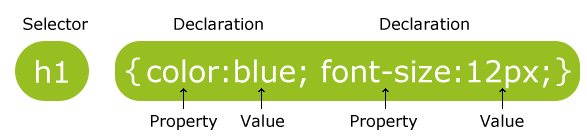
\includegraphics[height=0.25\paperheight]{fig/aula3/css_sintax.png} \\
    \tiny \textbf{Fonte:} \cite{freeman2008use}.
  \end{center}
\end{frame}
%-------------------------------------------------------------------------------
\begin{frame}{Sintaxe CSS}
  \begin{center}
    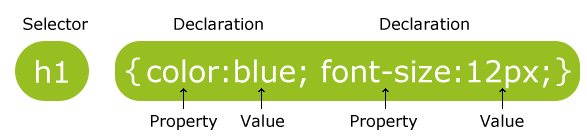
\includegraphics[height=0.25\paperheight]{fig/aula3/css_sintax.png} \\
    \tiny \textbf{Fonte:} \cite{freeman2008use}.
  \end{center}
\end{frame}
%-------------------------------------------------------------------------------
\begin{frame}{Inserindo estilo}
Inserindo um arquivo externo CSS.
  \begin{center}
    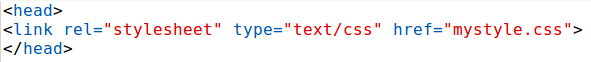
\includegraphics[height=0.12\paperheight]{fig/aula3/external_css.png} \\
    \tiny Link para folha de estilos
  \end{center}
  \begin{center}
    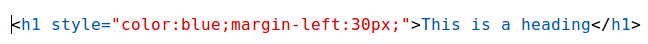
\includegraphics[height=0.08\paperheight]{fig/aula3/estilo_elemento.png} \\
    \tiny Estilo aplicado ao elemento
  \end{center} 
\end{frame}
%-----------------------------------------------------------------------------
\begin{frame}{Inserindo estilo}
Qual seria o resultado se para esta situação?
  \begin{center}
    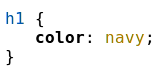
\includegraphics[height=0.2\paperheight]{fig/aula3/h1_css.png} \\
		  \tiny Na folha de estilos mystyle.css
	  \end{center}
	  \begin{center}
		  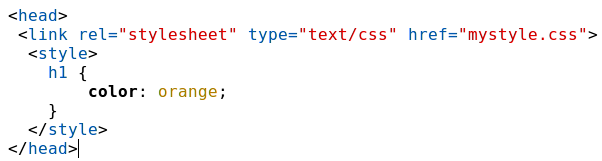
\includegraphics[height=0.3\paperheight]{fig/aula3/h1_html.png} \\
		  \tiny No HTML
	  \end{center}
	  
\end{frame}
%-----------------------------------------------------------------------------
\section{Seletores}
\begin{frame}{Elemento seletor}
  Os elementos Seletores são utilizados para estilizar elementos HTML.\\
  Ele encontra os elementos através do nome, id, classe e atributo.
  \begin{block}{Tipos de seletores*}
    \begin{itemize}
      \item Seletor elementos;
      \item Seletor id;
      \item Seletor classe;
    \end{itemize}
 \tiny *Os seletores apresentados são básicos, existem outros tipos de 
seletores.
  \end{block}
\end{frame}
%---------------------------------------------------------------------------------
\begin{frame}{Seletor Elementos}
Exemplo, seletor de elemento aplicado a $<p>$.
  \begin{center}
    \lstinputlisting{fig/aula3/elemento.css}
  \end{center}
\end{frame}
%---------------------------------------------------------------------------------
\begin{frame}{Seletor id}
Exemplo, seletor de elemento aplicado a um elemento com o id ``para1''.
  \begin{center}
    \lstinputlisting{fig/aula3/seletor_id.css}
  \end{center}
\end{frame}
%---------------------------------------------------------------------------------
\begin{frame}{Seletor classe}
Exemplo, seletor de elemento aplicado a um elemento definido com a classe ``center''.
  \begin{center}
    \lstinputlisting{fig/aula3/seletor_class.css}
  \end{center}
\end{frame}
%---------------------------------------------------------------------------------
\begin{frame}{Seletor classe}
É possível especificar que somente \textbf{um} elemento seja afetado por uma classe:
    \begin{center}
      \lstinputlisting[linerange={1-3}]{fig/aula3/seletor_class_element.css}
      \tiny Código HTML
    \end{center}
%   \vspace{0.2cm}
  \begin{center}
    \lstinputlisting[linerange={5-9}]{fig/aula3/seletor_class_element.css}
    \tiny Código CSS
  \end{center}
\end{frame}
%---------------------------------------------------------------------------------
\begin{frame}{Seletor classe}
É possível especificar \textbf{mais de uma classe} para um mesmo elemento:
  \begin{center}
    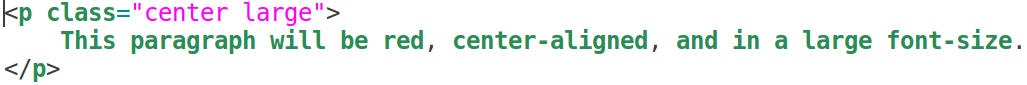
\includegraphics[height=0.1\paperheight]{fig/aula3/css2.png} \\
    \tiny Código HTML
  \end{center}
% 	\vspace{0.2cm}
  \begin{center}
    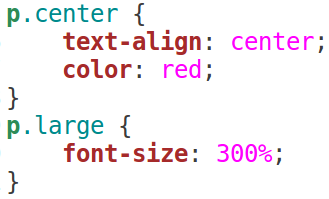
\includegraphics[height=0.2\paperheight]{fig/aula3/css1.png} \\
    \tiny Código CSS
   \end{center}
\end{frame}
%---------------------------------------------------------------------------------
\begin{frame}{Sobre Seletores...}
É possível agrupar seletores que possuem características iguais:
  \begin{columns}
    \begin{column}{0.4\textwidth}
      \begin{center}
	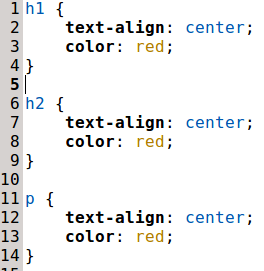
\includegraphics[height=0.45\paperheight]{fig/aula3/seletor_grupo.png} \\
	\tiny Seletores individuais
      \end{center}
    \end{column}
    \begin{column}{0.4\textwidth}
      \begin{center}
	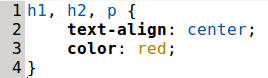
\includegraphics[height=0.15\paperheight]{fig/aula3/seletor_grupo1.png} \\
	\tiny Seletores agrupados
      \end{center}
    \end{column}
   \end{columns}
\end{frame}
%-----------------------------------------------------
\section{Cores e Background}
\begin{frame}{Nome de cores CSS}
	\begin{center}
			\lstinputlisting{fig/aula3/colors.css}
			\tiny Para mais cores consulte o \href{https://www.w3schools.com/colors/colors_names.asp}{link}.
		\end{center}
\end{frame}
%----------------------------------------------------------------------------
\begin{frame}{Utilizando Cores CSS}
É possível especificar a cor de vários elementos HTML.
	\begin{center}
		\lstinputlisting[linerange={1-1}]{fig/aula3/color_elements.css}
		\tiny Cor de fundo
	\end{center}
% 	\vspace{0.2cm}
	\begin{center}
		\lstinputlisting[linerange={2-2}]{fig/aula3/color_elements.css}
		\tiny Cor da fonte
	\end{center}
	\begin{center}
		\lstinputlisting[linerange={3-3}]{fig/aula3/color_elements.css}
		\tiny Cor da borda
	\end{center}
\end{frame}

%-----------------------------------------------------------------------
\section{Leitura recomendada}
\begin{frame}{Leitura complementar}
 Para mais informações sobre HTML e CSS, leia:\\
 \begin{columns}
   \begin{column}{0.5\textwidth}
    Desenvolvimento de Software II: Introdução ao Desenvolvimento Web com HTML, CSS, JavaScript e PHP \\
     Capítulo 4 - Página 61\\ 
      \cite{miletto2014desenvolvimento}
   \end{column}
   \begin{column}{0.3\textwidth}
    \begin{center}
  
\includegraphics[height=0.45\paperheight]{fig/aula3/milleto2014.jpeg} \\
 \end{center}
   \end{column}
 \end{columns}
\end{frame}
%--------------------------aula 4 des. app---------------------------------------------

\section{Referências}
\begin{frame}{Referências}%[allowframebreaks]
\frametitle{Referências}
\small
\begin{center}
\tiny
\bibliographystyle{apalike}
\bibliography{ref_aula}
\end{center}
\end{frame}
 
\end{document}
